%&latex
\documentclass[a4paper]{report}
\usepackage{commons/commons}
\usepackage{commons/note_style}
\usepackage{commons/code_style}
\usepackage[normalem]{ulem}
\usepackage{comment}
\usepackage{titlesec}
\titleformat{\chapter}[display]
  {\normalfont\sffamily\big\bfseries\color{black}}
  {\chaptertitlename\ \thechapter}{5pt}{\huge}
%\excludecomment{figure}
\usepackage{amsbsy}
\usepackage{amstext}

\graphicspath{{./fig/}}
\begin{document}

%+Title
\title{Advanced Algorithm Quicksheet}
\author{Daniel D. Zhang, \\ Based on \textit{Algorithm Design by Kleinberg \& Tardos}}
\date{Winter 2015. \today}
\maketitle
%-Title

%+Abstract
%\begin{abstract}
%This is the notes for CSE 232A.
%\end{abstract}
%-Abstract

%+Contents
\tableofcontents
%-Contents
\chapter*{Preface}
Quicksheet. It only contains the most essential information. 

You should read it accompanied with the book: \textit{Algorithm Design by Kleinberg \& Tardos}.
\section*{Acronyms}

\begin{obeylines}
\rih{Ptr}. Pointer
\rih{idx}. Access key to array, that is array index; but it is not the database index.
\rih{est}. Estimate.
\rih{$\bot$}. Independent.
\rih{CNP}. Converse-negative proposition

\end{obeylines}

\section*{Proof techniques}
Algorithmic problem solving.
\begin{enumerate}
\item ideas
\item math notations: declarative rather than procedural. - don't think about the implementation details. Think about mathematical expressions (\textit{Functional Programming} way of thinking). 
\item numbering 
\item correctness proof 
\item time complexity derivation 
\end{enumerate}
Basic components of developing algorithm problem solutions:
\begin{enumerate}
\item Classification of problems
\item Trial ideas 
\item Draft procedure
\item Proof of correctness
\item Write formal solution
\end{enumerate}
Basic components of writing algorithm problem solutions:
\begin{enumerate}
\item Procedure 
\item Correctness
\item Time complexity
\end{enumerate}
\chapter{Introduction}
\section{Iterative Improvement - Stable Matching Problem }
Techniques.

Example: Stable Matching Marriage. People with free-will. 

Definition of \textbf{stability}:
Dataset: $w_1, w_2, m_1, m_2$.
\begin{align*}
w_1: m_1 > m_2\\
w_2: m_2 > m_1\\
m_1: w_2 > w_1\\
m_2: w_2 > w_1\\
\end{align*}
Stable matching pair: $m_i$ same preference, thus, $w_i$ gets the choices. 
\chapter{Divide \& Conquer}
\section*{Discussion - tree \& complexity}

Algorithm, starts from high-level, iterative refinements. 

MergeSort example: 

Divide procedure: 
Split the array $X$. Rough information: middle. Precise notation: $\lfloor\frac{n}{2}\rfloor$.

Merge procedure: 

Result invariant - non-decreasing. Taking the smaller element from the two sorted lists.

Corner case and base cases are important. 

\begin{align*}
T(1) &= 1\\
T(n) &= T(\lfloor \frac{n}{2}\rfloor) + T(\lceil \frac{n}{2}\rceil) +n \\
T(n) &= 2T(n/2)+n\\
T(n) &= 2(2T(n/4)+n/2)+n \\
\end{align*}

Let $n$ be a power of 2. 

Recursion tree method. Tree levels, tree nodes. 

Level $k$, $k=\lg n$. 

Reasoning process: 

Level - \# nodes per level - size per node - cost per node - cost per level

Precise answer:
$$
n (\lg n + 1)
$$

Variant: 
\begin{align*}
T(n) &= 2T(n/2)+2n \\
T(n) &= 3T(n/3)+n
\end{align*}
\begin{tabular}{lllll}
\hline\noalign{\smallskip}
\textbf{level} & \textbf{\#nodes per level} & \textbf{size per node} & \textbf{cost per node} & \textbf{cost per level}\\
\noalign{\smallskip}\hline\noalign{\smallskip}
0 & 1 & n& n &n \\
k & 3^k & n/3^k & n/3^k &n\\
\log_3 n & ...\\
\noalign{\smallskip}\hline\noalign{\smallskip}
\caption{Recursion tree}
\end{tabular}

Variant:
$$
T(n) = 3T(n/2)+n
$$
\begin{align*}
\sum_{k=0}^{\lg n} 3^k \frac{n}{2^k} \\
& = n \cdot 1.5^{\log_2 n} \\
&= n^{1+\log_2{1.5}} \\
&= n^{log_2 {3}}
\end{align*}


For increasing geometric sequence, keep the \textbf{last} term; for the decreasing
one, keep the \textbf{first} term.

\begin{align*}
T(n) = 4T(n/2)+n^2 
\end{align*}
\begin{tabular}{lllll}
\hline\noalign{\smallskip}
\textbf{level} & \textbf{\#nodes per level} & \textbf{size per node} & \textbf{cost
per node} & \textbf{cost per level}\\
\noalign{\smallskip}\hline\noalign{\smallskip}
0 & 1 & n& n &n \\
k & 4^k & n/2^k & (n/2^k)^2 &n^2\\
\log_3 n & ...\\
\noalign{\smallskip}\hline\noalign{\smallskip}
\caption{Recursion tree}
\end{tabular}

\section*{Discussion - stable matching and D\&C}
\subsection*{Truthfulness}
Stable Matching: lie to improvement self utility.

Follow the books the convention that men propose. Lying, it is possible to degenerate own outcome. Does lying always improve the utility? 

GS algorithm 1 dof: which free man to propose in \pyinline{while} loop. After proof, it always produces the SAME stable matching. Thus, it is possible to always improve by lying. 

\subsection*{Men-optimal}
Proposition: each man get the\textbf{ best stable} partner. Each woman get the \textbf{worst stable} partner. 

Proof by contradiction: $\exists m\in M$ does not get the best stable partner; thus he was rejected by the best stable partner. Chronologically, consider the first man rejection during the execution time. 

In matching $S$, $S$ is produced by GS:
\begin{align*}
& m-w'\\
& m'-w\\
& m: w >w'\\
& w: m' > m\\
&m': w > w''
\end{align*}

In $S'$: 
\begin{align*}
& m-w\\
& m'-w''
\end{align*}
, where $\exists w\in W, w=bestStable(m)$ is the best stable for $m$. 



Goal: $m'... w$ is a blocking pari in $S'$; thus $S'$ is not valid; thus to prove that $w\neq bestStable(m)$. 

Another level of proof by contradiction: 
Assume $m': w'' >w$. Then $m'$ proposes to $w''$ but rejected, which contradicts the $m$ is the \textbf{first} rejection. Thus, $m': w>w''$. Thus blocking pair in $S'$

\subsection*{Local Minimum}
$m*n$ matrix. $N=\max(m, n)$

\subsubsection*{Follow your nose} 
\textit{Follow your nose} algorithm: start with any cell \pyinline{cur}, if it is a local min, found; else, at least one \pyinline{cur < nbr}, then \pyinline{cur = nbr}. - Iterative improvement. 

Does it terminate? There is no infinite loop $\infty$, proof by contraction, some cell strictly $>$ itself.

When it terminates, it found because all conditions met. 

This algorithm proves the existence of the local minimum. But this algorithm is $O(mn)$.
\subsubsection*{Improvement}
Binary search in 1d, divide into 2 parts. Binary search in 2d - divide into 4 parts. 
Check the border of 4 parts (squares). 

The sub-problem must have exact pattern and only differs in size. And we want to have balanced parts rather than size-unbalanced parts. 

When if we found local min in a part on the border of the part, can we ensure this local min is actually the local min considering the boundary that is thrown away when entering into this part. Thus, what we need is a clean cut. 

\subsection*{Hidden surface}
Do the analogy. 
Compared to \textbf{merge sort}, this problem has no clear input and data structure (repr). Visible surface is abstraction without concrete data structure. What is the data structure used to repr the visible surface. What you are merging the visible surface. 

$L_1, ..., L_n$ repr as:
$$
y=m_ix+b_i
$$

To repr the visible surface: indexes of lines give the \textbf{sequence} to calculate the intersecting point $\in$ surface. 

In the merge sort, there are two increasing sequences. What are  the ``increasing'' surfaces? Then how to merge the two ``increasing'' surfaces?

END OF DISCUSSION

\section{Integer Multiplication}
D\&C. 
\begin{align*}
& (x_1 2^l+x_0)(y_1 2^l+y_0)  \\
=& x_1y_12^{2l}+x_1y_02^l+x_0y_12^l+x_0y_0
\end{align*}
Calculate 3 parts instead of 4 parts. 
\begin{enumerate}
\item $x_1y_1$
\item $x_0y_0$
\item $(x_1+x_0)(y_1+y_0)=x_1y_1+x_1y_0+x_0y_1+x_0y_0$ 
\end{enumerate}
\section{FFT}
From integer multiplication to polynomial multiplication 
\begin{align*}
& A(x) = \sum_{i=0}^{n-1} {a_i x^i}\\
& B(x) = \sum_{i=0}^{n-1} {b_i x^i}\\
& C(x) = A(x)*B(x) = \sum_{i=0}^{2n-2} {c_i x^i} \\
& \text{, where } c_i = \sum_{j=0}^i {a_j b_{i-j}}
\end{align*}
Notice that sum of indexes is the same.

Fourier transformation: frequency domain $\leftrightarrow$ time domain. Coefficient domain $\leftrightarrow$ value domain. 

Eval $A(x), B(x), C(x)$ using $x_1, ..., x_n$. And you have the freedom of choosing $x_i$. You can evaluate the expressions when  $x_i=1$ and $x_i=-1$, you can easily eval; $\Ra$ we want $\forall i, x_i$ is 1 or -1. 
\subsection{General Form}
General form of FFT. Books use the index that starts at 0. 
\begin{align*}
\vec c &= \vec a*\vec b \\
\vec c_k &= \sum_{(i,j): i+j=k} \vec a_i\vec b_j\\
|\vec c| &= |\vec a|+|\vec b| -1 
\end{align*}
It is the 1-d convolution, which is exactly the same as 2-d convolution except that the dimension has increased. 

Take middle part (\textbf{subset}) of $\vec c$:
$$
\vec c'_k =\sum_{(i,j): i+j= k+n} {\vec a_i \vec b_j}
$$

\section{Closet pair}
\begin{figure}[!htp]
\centering
\subfloat{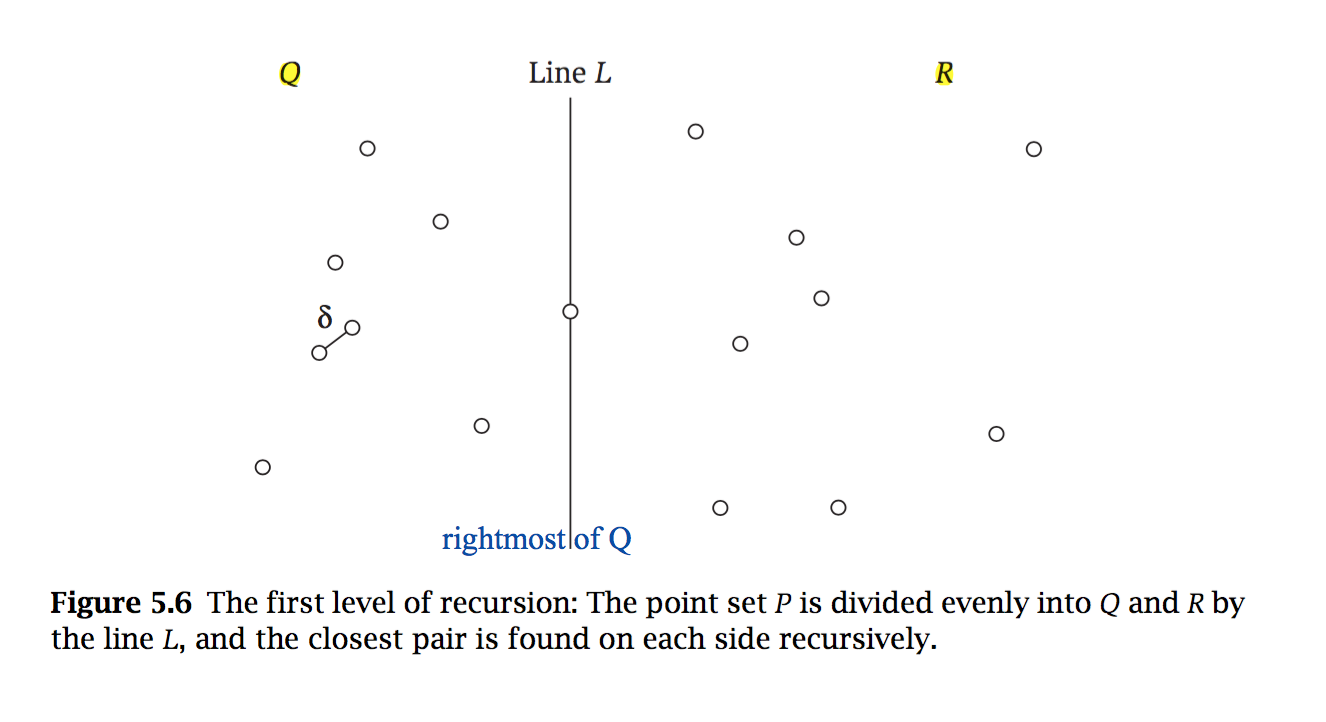
\includegraphics[scale=1.30]{5_6}}
\caption{Divide}
\label{fig:5_6}
\end{figure}
Find a closet pair in graph: 

$(x_i, y_i), 1\leq i \leq n$. Find $i\neq j$ s.t. $(x_i-x_j)^2+(y_i-y_j)^2$ in min.

\subsection{1-D problem} 
Sort and compare neighboring points. 

\subsection{2-D with a narrow band}
Naive sort by $x$-coordinate, counter example: $(0, \delta), (\varepsilon,-\delta), (2\varepsilon,\delta)$

Slight deviation from the 1-D line. All points fall in a strip $2\delta$. 

But can the $\delta$ be far apart? Try to figure out the upper limit of $\delta$.

After getting $\delta$, divide the band into cells of length $\delta$. 
\begin{python}[mathescape]
----------
|_|_|_|_|_| $\delta$
| | | | | | $\delta$
----------
\end{python}

We need to find the closet pair in this narrow band, We stuck here for finding close pair in band because we haven't define the \textit{algorithmic meaning} of $\delta$, 

\subsection{2-D D\&C} 
\begin{figure}[!htp]
\centering
\subfloat{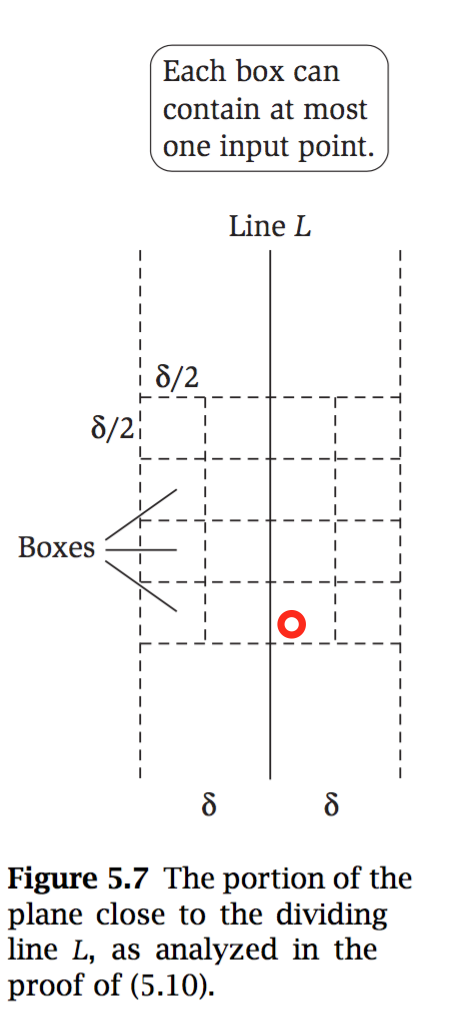
\includegraphics[scale=1.30]{5_7}}
\caption{Check neighboring points within the brand.}
\label{fig:5_7}
\end{figure}
Target: total $O(n \lg n)$, merge $O(n)$. 

$\delta = \min(\delta_1, \delta_2)$, where $\delta_1$ is from the right sub-problem, and $\delta_2$ is from the left sub-problem. 

Does there exist a pair of point $l \in \mat{L}, r \in \mat{R}$, s.t. $d(l, r) <\delta$. 

\textbf{FILTER} out the impossible (informational useless) points. 
\begin{enumerate}
\item \textbf{Outside the band}: require $d(l, r)<\delta \Ra$ filter out points reside outside the separating line $L$ band of $\pm\delta$ (rather than $\pm0.5\delta$) along the $x$-axis. Form the band $\mat{S}$. 
\item \textbf{Inside the band}: require $d(l, r)<\delta \Ra$ for each scanning point $cur$,  filter out points reside outside the $\pm\delta$ along the $y$-axis; only keeps neighbors. \textbf{Limited search space}. After filtering, find the upper bound of number of neighboring points.  
\end{enumerate}

If you divide the band into finer cells of length $\frac{\delta}{2}$. For each point $cur$, there are only $O(16-1)$ points that is possible to have $d(cur, nbr)<\delta$ within the 16 neighboring cells respectively. $+4: 4^2$. Then reduce the search space into $O(16-1)$ along the $y$-axis. Notice that $\forall cell$, at most 1 point $\in cell$ due to the $cell \in \mat{L}$ or $cell \in \mat{R}$.

Although unnecessary, we can further reduce the search space, if the $cur\in \mat{L}$, no need consider $\{nbr|nbr\in \mat{L}\}$, the only need to consider $4^2/2=8$ neighbors, up 4 and down 4. Thus need to compare 8 $nbr$ in $S_y$. 

\subsection{Writing Proof}
How to write the proof:
\begin{enumerate}
\item High-level ideas
\begin{enumerate} 
\item \textbf{Notations}. Define the mathematical notations rigorously. 
\begin{enumerate}
\item Let $S_L' = \{p|p\in S_L, |p_{x}-x_{mid}|\leq \delta) \}$, where $p_x$ is the
$x$-coordinate of $p$.
\end{enumerate}
\item  \textbf{High-level}. The detailed can be suppressed since assume background knowledge. Thus, provide high-level details rather than implementation details
\begin{enumerate}
\item ``while keeping track of the $min$''.  
\item Let $S_L$ sorted by $x$-coordinate in
what order.
\end{enumerate}
\item \textbf{Sections}. e.g. D\&C - 1) base case 2) divide 3) merge 
\end{enumerate}
\item Proof
\begin{enumerate}
\item \textbf{Target}. What we found is what we want. - the target is only in the subsets; why we can
filter out other sets.
\item \textbf{Numbering} Numbering the arguments in the ideas, easier to ref.
\end{enumerate}
\item Time complexity
\begin{enumerate}
\item \textbf{Track}. Track and argue the time complexity. [$O(N)$]
\item \textbf{Recursion}. Solve the recursion equation 
\item \textbf{Const}. Constant matters
\item \textbf{Graph}. Verbal is necessary while graph is not sufficient, although graph assists the math notations. 
\end{enumerate}
\end{enumerate}

\subsection{Dimension}
for high dim data points:
$$
2^k n \log n 
$$
\section{Majority element}
find $x$ in array $A$ with length $n$ s.t. $cnt_x > n -cnt_x$. 

Find a pair $(a_i, a_j)$ in $A$, if $a_i \neq a_j$, delete both from $A$. it still holds that: $C^{A'}_x > |A'|-C^{A'}_x$. Proof, since $a_i\neq a_j$, at most 1 of them equals $x$, then $C^{A'}_x$ decrements at most by 1, $|A'|$ decrements by 2. 

To find such pair $(a_i, a_j), a_i\neq a_j$, linear time one-pass algorithm. That's why \textit{Moore's voting algorithm} is correct. 

Proof: At any time in the execution, let $A'$ be the prefix of $A$ that has been processed, if $counter>0$, then keep track the candidate $majority$'s counter, the $majority$ is the majority number of $A'$.  If $counter =0$, then for $A'$ we can pair the elements s.t. are all pairs has distinct element. Thus, it does not hold that $cnt_x>n-cnt_x$; thus $majority\in A'$.

What if there no majority number. Proof the relaxed problem (i.e. majority number must exists) as above; then handle stricter problem. 

\textbf{D\&C}. Need to keep track the number of matched pair; need to handle the odd-length subset $\Ra$ more complicated. 

Why simple find the majority in subset is not sufficient: 7 $x$, 6 $y$. 
\begin{align*}
[(x, x) (x, x) (y,x)][(y, x) (y, x) (y, y)][y]
\end{align*}

After conquer:
\begin{align*}
x | y|y
\end{align*}
\subsection{Skyline}
Similar to visible surface, but easier. 

\textbf{repr}. Define the repr. The number of building is $n$. The building is represented in $(s_{i}, e_{i},h_{i})$, s.t. in the interval $[s_i, e_i)$, the height is $h_i$. 

What is the repr for the skyline? A list = $[(s'_i, e'_i, h'_i)]$


Use D\&C. When the skyline changes? At start and end. 

\textbf{Preprocess}. Sort the building by $s$. 

\textbf{Divide}. Divide into $B_1, B_2$ and conquer them. 

\textbf{Merge}. Merge efficiently $B^1, B^2$, scan the $x$ from either $B^1, B^2$, $h_x$ at $x$ is $h_x=\max(h^1_x,h_x^2)$. Sorting building by $s$ can make it easier. Use $e^1_{end}$ and scan the points from $B^2$

\chapter{Greedy Algorithm}
Agenda:
\begin{enumerate}
\item Scheduling max number of intervals 
\item Minimizing max lateness
\item Cache replacement policy
\end{enumerate}
Techniques:
\begin{enumerate}
\item Exchange method 
\begin{enumerate}
\item Compare $\mat{G}, \mat{O}$. 
\begin{enumerate}
\item Starts from head, the 1st one 
\item Starts with the immediate neighbors, inversion. 
\end{enumerate}
\end{enumerate}
\item Stays ahead method
\begin{enumerate}
\item Compare $\mat{G}, \mat{O}$
\item Mathematical induction 
\end{enumerate}
\end{enumerate}
\section{Events scheduling}
\textbf{Definition} of the problem: Max number of intervals without overlapping. 

\textbf{Notations}
$$
[s_i, f_i), \text{ where }0 \leq i < n
$$

\textbf{Ideas}
\begin{enumerate}
\item select the interval with min degree of conflicts 
\item select the interval with shortest duration 
\item select the interval with min start time 
\item select the interval with min end time
\item select the interval with latest start time (dual with 4, same as 4 and just look a the input arrays in a reversed order)
\end{enumerate}

\textbf{Proof} idea 4. Proof by contradiction and proof by induction. Greedy solution $\mat{G}$, optimal solution $\mat{O}$. 
\begin{align*}
& \mat{G} = \{G_0, G_1, ..., G_{k-1}\}  \\
& \mat{O} = \{O_0, O_1, ..., O_{l-1}\} \\
& k > l 
\end{align*}

Sort $\mat{G}, \mat{O}$  by finish time. 

Technique ``\textit{Exchange Method}". rearrange the $\mat{O}$ to look like $\mat{G}$, and to the end $\mat{O}, \mat{G}$ are the same (i.e. $|\mat{O}|=|\mat{G}|$). 

For the 1st elt:
\begin{enumerate}
\item if $G_0=O_0$, then move to the next index
\item else, $G_0.f < O_0.f$ since greedy; and then exchange $O_0$ with $G_0$ without conflicting other $\mat{O}[1:]$.

There is no conflicting in $\mat{)}[1:]$, because $\forall i\geq 1, O_i.s > O_0.f >G_0.f$. 
\end{enumerate}

For the 2nd elt: Since after exchange, $G_0=O_0$, we truncate the first element, thus the problem $\mat{O}[1:], \mat{G}[1:]$ can be solved similar as  $\mat{O}[0:], \mat{G}[0:]$.

After iteratively applied, $\mat{G}[0:k]=\mat{O}[0:k]$.

After consuming all the $k$ element, the way of greedy works (select the earliest end time \textit{until} there are no more), (you need to argue that) there is no more $O_{k},..., O_{l-1}$. If there are more, the greedy algorithm will continue the selection which contradicts that the greedy has stopped.

\section{Exercise}
General methods to proof greedy algorithm
\begin{enumerate}
\item Exchange method
\item Stay head 
\item Optimal substructure - for dp. 
\end{enumerate}
\subsection{Changing road conditions}
\begin{align*}
& G_i \ra G_{i+1}\\
& P_i \\
& G_i, P_i, \sum_{i=0}^b l(P_i)+K \cdot change(P_0, ..., P_b)
\end{align*}
, where $k$ for the penalty of changing the path. 

The $t$ changes, but the previous path does not change, but it may not be the shortest path. 

Cannot to D\&C since the two subproblems (divide the Graph into two halves) influences each other. There is no clear boundary btw two subs. 

\textbf{Relexation}. Take a simpler version of the problem, regardless the previous sequence, for the subsequent subs, you get the min cost. Define substructure with parameters to relax problem. 

\textbf{Solution}. The effect of $G_i$ on the earlier part is hard to anticipate in a greedy-type algorithm, so we'll use dynamic programming. 

\subsection{Timing circuits}
Data structure. Goes up \& down. repr
\begin{enumerate}
\item Pointers
\item Heap (heapq)
\end{enumerate}

BFS, and set the length. 

Don't need to write pseudo-code. 

Ideas:
\begin{enumerate}
\item start at leaf level. 
\item start at root level.
\end{enumerate}

Produces $\forall$ root-to-leaf path lengths are equal (intermediate nodes doesn't matter) and with min sum of edge lengths. 

Observations: 
\begin{enumerate}
\item The greedy algorithm produces the with zero-skew result s.t. the root-to-leaf path length equal to the maximum root-to-lead path length; and minimal length. The extra property is - max original root-leaf path. 
\item defining this additional property that can do \textit{recursion}.
\end{enumerate}

Procedure: 

1 level down, make two trees rooted at left child and right child be min-zero-skew-max-length trees; and adjust root to left and right child length to the the max-length from root-leaf path. 


Proof the correctness of idea: refer to homework. 

\subsection{Time-varying MST}
Kruskal's algorithm is sufficient. less complex than Prim's.

Exploit Kruskal's algorithm property that. 

Find the changing points (calculus). between the changing points, the relative order of the $E$ does not change. 

Once the order changes, re-run the Kruskal. (no need to optimize). Just need polynomial algorithm. 

The problem is reduced to find the changing points. 


\section{Optimal substructure}
\textit{Proof technique} for greedy algorithm and dp.

a problem is said to have optimal substructure if an optimal solution can be \textbf{constructed} efficiently from \textbf{optimal} solutions of its \textbf{subproblems}. This property is used to determine the usefulness of dynamic programming and greedy algorithms for a problem.

e.g. maxima number of intervals. 

Find optimal solutions in subproblem, and combine the the solution. 

\section{Minimize Max Lateness}
Tasks $(t_i, d_i)=$ (duration, deadline). 

Schedule $(s_i, f_i)$, where $f_i=s_i+t_i$, start time and end time. All jobs can be scheduled. The goal is to minimize the max lateness: 
$$
\min L = \min(\max_i l_i), \text{ where } l_i=\max(0, f_i-d_i)
$$

Analysis: 1st observation, no reason for gaps between tasks.

\textbf{Ideas}: Greedy, at current step:
\begin{enumerate}
\item select min $d_i$ first
\item select min $t_i$ first, counter example: $(2, +\infty)$, $(2, 2)$
\item select max $l_i$ first 
\end{enumerate}

\textbf{Strategy}:

\textbf{Proof}. The correct answer is take min $d_i$ first. 

Prof by contradictions + \textit{Exchange Method}

Consider the greedy solution $\mat{G}$ s.t. scheduled as $d_1 \leq d_2\leq ...$. Consider a opt solution $\mat{O}, \exists i,j, d_i > d_j$ s.t. $i$ is scheduled earlier. 

$\Leftarrow$ Exchange method: exchange $i, j$, but hard to analyze for the schedules $\mat{O}[i+1:j]$. However, If $i, j$ is \textbf{adjacent}, it is easier.
\begin{figure}[!htp]
\centering
\subfloat{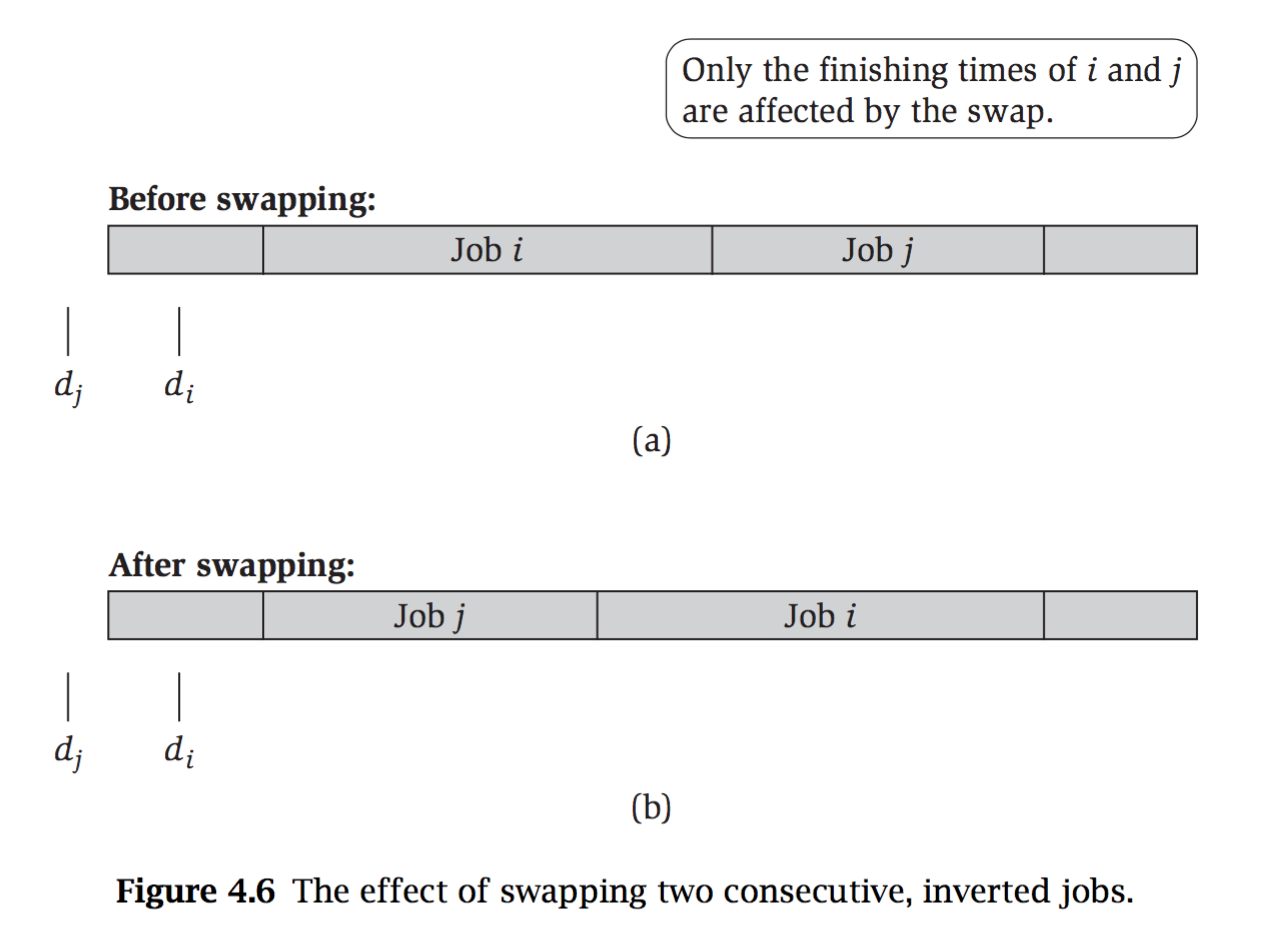
\includegraphics[scale=1.0]{4_6}}
\caption{Consecutive intervals}
\label{fig:4_6}
\end{figure}

Define before swapping, the schedule is $\mat{O}$, after $\mat{O'}$. In $\mat{O'}$, job $j$ is earlier than in $\mat{O}$, lateness can only be reduced. Only need to prove $l_j>l'_i$.
\begin{align*}
& \mat{O} \text{ is worse than } \mat{O'} \\
\Leftarrow & \max(l_j, l_i) > \max(l'_j, l'_i) \\
\Leftarrow & \because l_j > l'_j; \because \max.  \therefore \text{only need to prove } l_j>l_i'
\end{align*}
When have one important equality: $f_j=f'_i$ (draw the diagram). 
\begin{align*}
& l_j > l_i'\\
\Leftarrow & f_j - d_j >f_i'-d_i \\
\Leftarrow & f_j - d_j >f_j-d_i \\
\Leftarrow & d_j < d_i
\end{align*}

Lateness of job j in $\mat{O}, l_j= f_j - d_j$

Lateness of job j in $\mat{O'}, l'_j= f'_j - d_j$

$l'_i=f'_i - d_i=f_j-d_i$. Thus, $l'_i<l_j$



\begin{align*}
&\because l_j > l'_j, l_j>l'_i\\
\end{align*}

Here it does not consider $\exists j, d_j>f_j$

Then like bubble sort to swap the nodes.

We say that a schedule has an \textit{inversion} if a job $i$ with deadline $d_i$ is scheduled \textbf{before} another job $j$ with \textbf{earlier} deadline $d_j<d_i$.

The optimal solution is the one with no inversions. If $\mat{O}$ has an inversion, then $\exists$ a pair of jobs $i$ and $j$ s.t. $j$ is scheduled immediately after $i$ and has $d_j<d_i$. $\blacksquare$

\section{Min cost of pair-wise sum}
Operation: Sum pair-wise 

Sum all. Goal: get the minimize cost $c\triangleq A_i+A_j$.

Analysis:

Take 2 min elements, and sum them up, del the 2, put back the sum. Repeat this process.
Thus, use heap. 

Proof. \textit{Exchange method}, $\mat{O}, \mat{G}$ consider an inversion point. 

\section{Relationship with DP}
DP is the superset of Greedy. 
\chapter{Dynamic Programming (DP)}
\section{General}
\begin{enumerate}
\item Forward (prefix) dp $[:i]$, backward (suffix) dp $[i:]$
\item End with $i$ (required); End before or with $i$ (optional)
\item Expand parameters of the state $F$ to refine the substructure
\item From different perspective 
\begin{enumerate}
\item Consumed vs. Remaining 
\item Assigner vs. Assignee 
\end{enumerate}
\end{enumerate}
\section{Interval Scheduling with Weights}
Given intervals $A$: $[s_i, f_i), w_i\geq 0$, where $w$ is the weight. 

The state definition is to redefine the problem. 

\textbf{State definition}:
$M_i=$ max sum of weights of a non-overlapping set of jobs where the jobs come from $A[i...n]$

Least relaxed problem: $M_1$. Most related problem $M_n$.

\textbf{State transition functions}: Basically you have two choices: 
\begin{align*}
M_i = \min&\Big( w_i+M_j \text{, where $j$ is the earliest index s.t. } s_j\geq f_i\\
&M_{i+1}\Big)
\end{align*}

Earliest index math definition: $j=\min\{j>i|s_j\geq f_i\}$. It is possible that $j\in \phi$. 


Notice that, $M(i)$ is monotonous.

Suffix intervals 

Formal math def:
\begin{align*}
& \text{State definitions} \\
& Next(i) = \{j>i|s_j\geq f_i\}\\
& N_i = \min Next(i) \text{ if } Next(i)\neq \phi \text{ else } None\\
& M_i = \text{Max sum of weights for interval $i$ through $n$} \\
& D_i = 1 \text{ if interval $i$ is included in the optimal solution for interval $i$ through $n$; else } 0\\
\\
&\text{Initialization}\\
& M_{i}=W_n \\
& D_n=1 \\
\\
&\text{State transition} \\
&\text{for i = n-1 downto 1:}\\
& M_i = \max\Big(w_i+M_{N_i} \text{ if }N_i\neq None \text{ else } w_i, \\&
\quad M_{i+1} \Big) \\
& D_i = 1 \text{ if }w_i+M_{N_i}\geq M_{i+1} \text{ or } w_i \geq M_{i+1} \\
& \quad 0 \text{ ow} \\
& \text{Output the optimal solution} \\
& out(1)\\
\end{align*}
\begin{python}[mathescape]
def out(i):
  if $D_i=$ 1:
    output interval $A_i$ 
    if $N_i\neq$  None:
      out($N_i$)
  else:
    out(i+1)
\end{python}

The notations should be well defined. 


\section{DP computing}
solve the problem in brute force, find same subs, cache them, reduce exponential to polynomial. 
\subsection{Cached recursion}
\subsection{Tabulation}
\section{Segmented Least Squares}
input: $(x_i, y_i), 1\leq i\leq n$ output: $a, b$ for $y=ax+b$. 

Why take square of the error? make the cost function to be convex to use gradient descent. 
Fit lines, two extreme cases:
\begin{enumerate}
\item 1 line 
\item lines on every consecutive pair 
\end{enumerate}

Rough thoughts:
$$
\varepsilon_i = \min_{j\in (i, n]} \Big(LSE(i, j)+\varepsilon_j\Big)
$$

Regularization using \textbf{penalty} $\mat{P}$, $\mat{P}$ can also be a function. 
$$
\varepsilon_i = \min_{j\in (i, n]} \Big(LSE(i, j)+\varepsilon_j+\mat{P}\Big)
$$
\begin{figure}[!htp]
\centering
\subfloat{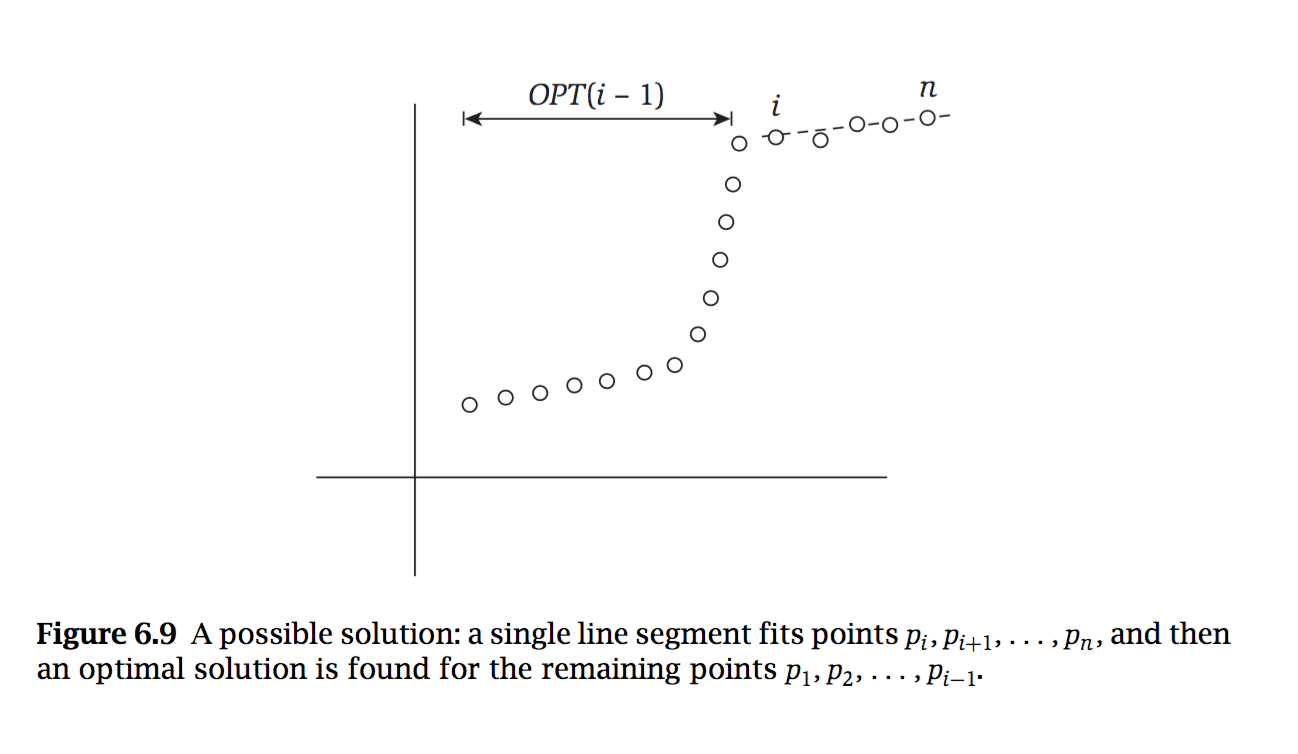
\includegraphics[scale=1.30]{6_9}}
\caption{Segmented Least Squares}
\label{fig:6_9}
\end{figure}
General forms:
$$
F_i = \min_{j\in(i,n]}\Big(F_j+\mat{C}(i, j)+\mat{P}\Big)
$$
, where $\mat{C}(i, j)$ is the cost of transition from $i$ to $j$, and $\mat{P}$ is the penalty. 

\section{RNA Secondary Structures}
TODO Graph

Target: fold told the linear chain to \textbf{folded} line. determines a secondary structure S with the maximum possible number of base pairs.

Rule of fold
\begin{enumerate}
\item No pinch 
\item Matching 
\item Non-crossing (this actually define a clear \textbf{boundary} to divide into subproblems)
\item $A \leftrightarrow U, G \leftrightarrow C$
\item $(i, j), (k,l) \ra (i<j<k<l \equiv (k-i)(l-j)>0)$
\end{enumerate}
The non-crossing condition is actually a help rather than the obstacle. 

Math notations:
$\Sigma=\{A, U, G, C\}$

Let $a_1, ..., a_n\in \Sigma^*$

output a sequence of pair $(i, j)$ s.t. 
\begin{enumerate}
\item $i<j$
\item $|j-i| > 4$
\item $(a_i, a_j)\in \mat{M}$, where $\mat{M}= \{(A, U), (U, A), (G, C), (C, G)\}$. 
\item Each index $i$ can only appear at most in one pair. 
\end{enumerate}

Can be thought recursively. 

\textbf{First} attempt $F_j$, after pair $(j-1, t)$, $F_i$ fails to capture the substructure of $A[t:j-1]$

\textbf{Second} attempt: Let $F_{i,j}$ be the max possible number pairs in $A[i:j]$.

When $j-i<5$:
\begin{align*}
F_{i, j} = 0
\end{align*}

For the current scanning index $j-1$, have two options pair $(j-1, t)$ or not. 

\begin{align*}
F_{i, j} = \max\Big(&F_{i, j-1}, \\
& \max_{(t, j-1) \in \mat{M} \wedge j-1-t>4} (F_{i, t}+1+F_{t+1, j-1})\Big)
\end{align*}

Notice that you can do either forward dp or backward dp. 

\section{Midterm}
\subsection{Median}
\subsection{Restaurant}
Let $M_i$ be the max profit obtained with restaurant opened at position $i$ through $n$. (suffix)
\begin{align*}
M_i = \max_{j>i+d(i)} \Big(P_i + M_j\Big) 
\end{align*}

Calculate the 
$$L_i=\min_j\{j>i|d_j - d_i \geq k\}$$

\textbf{Efficient} way to compute the $L_i$

But $M_i$ is \textbf{decreasing} array, thus only need to find the $L_i$.
$$
M_i = p_i + M_{L_i}
$$

TODO: efficient way. f
\subsection{Class Assignment}
The order of the classes does not matter. The strategy: find the smallest available room. 

\textbf{Proof} the correctness of the strategy. 

\textit{Exchange method}. Fixed the order of classes. 
$C(\alpha)\geq S(\alpha)$. 

$\mat{G}=\{R_1,R_2, ..., R_n\}$, where $\forall i, C(R_i)\geq S(i)$. 

$\min \sum_{i=1}^n C(R_i)$. 

Assume a optimal produces $\mat{O}=\{R_1', R_2', ..., R_n'\}$ with a smaller sum. 

Assume $R_1$ appears in $\mat{O}$ as $R_j'$. 
\begin{align*}
& C(R'_1)\geq C(R_1) \text{ since greedy way}\\
& \because C(R'_1)\geq C(R_j') \geq S(R_j') \wedge C(R_j')\geq S(R_1) \therefore \text{Can swap } R_1',  R_j'\\
& \text{Consequently, after swapping,}  \mat{O}[0]=\mat{G}[0]
\end{align*}

Uniter intervals cover the houses. Greedy method: left endpoint just cover the 1st house, then remove all covered houses. 

\textbf{Proof.} Exchange method. Focus on the 1st house. In $\mat{O}$ the interval is to the left of that of $\mat{G}$ then can exchange. 

\chapter{Network Flow}
\section{Max Flow - Min Cut}
\subsection{Notations}
Max Flow: highly abstracted model. 
\begin{enumerate}
\item Discreted graph $G=(V,E)$
\item Vertices $u, v, u_i, v_i, s, t$
\item Edges $e, e_L, (u,v), uv$
\item Capacity $C: E\ra \R, C(e)$. (it is not weight)
\item Flow: $f: E\ra \R$
\end{enumerate}
Properties 
\begin{enumerate}
\item $\forall e \in E, 0\leq f(e)\leq C(e)$
\item Conservation: $$\forall v\in V/\{s,t\}, \sum_{uv\in E}f(uv)=\sum_{vu\in E}f(vu)$$
, where $uv$ is the inflow for $v$, and $vu$ is the outflow. Compact notation $f^{in}(v), f^{out}(v)$. 
\item The Value of the graph:
$$V(f) = \sum_{su\in E}f(su)$$
, outflow for $s$. 
\end{enumerate}
Target: find $f$ with $\max V(f)$.

Idea: 
\begin{itemize}
\item Try greedy algorithm does not work
\item Need to undo the flow
\item Residual graph to allow undo for the flow. 
\item Backtrack is normally exponential, but it need to be done in an efficient way. 
\end{itemize}
\subsection{Ford-Fulkerson Algorithm}
\subsection{Residual Graph}
$G_R$ - Residual Graph 
\begin{figure}[!htp]
\centering
\subfloat{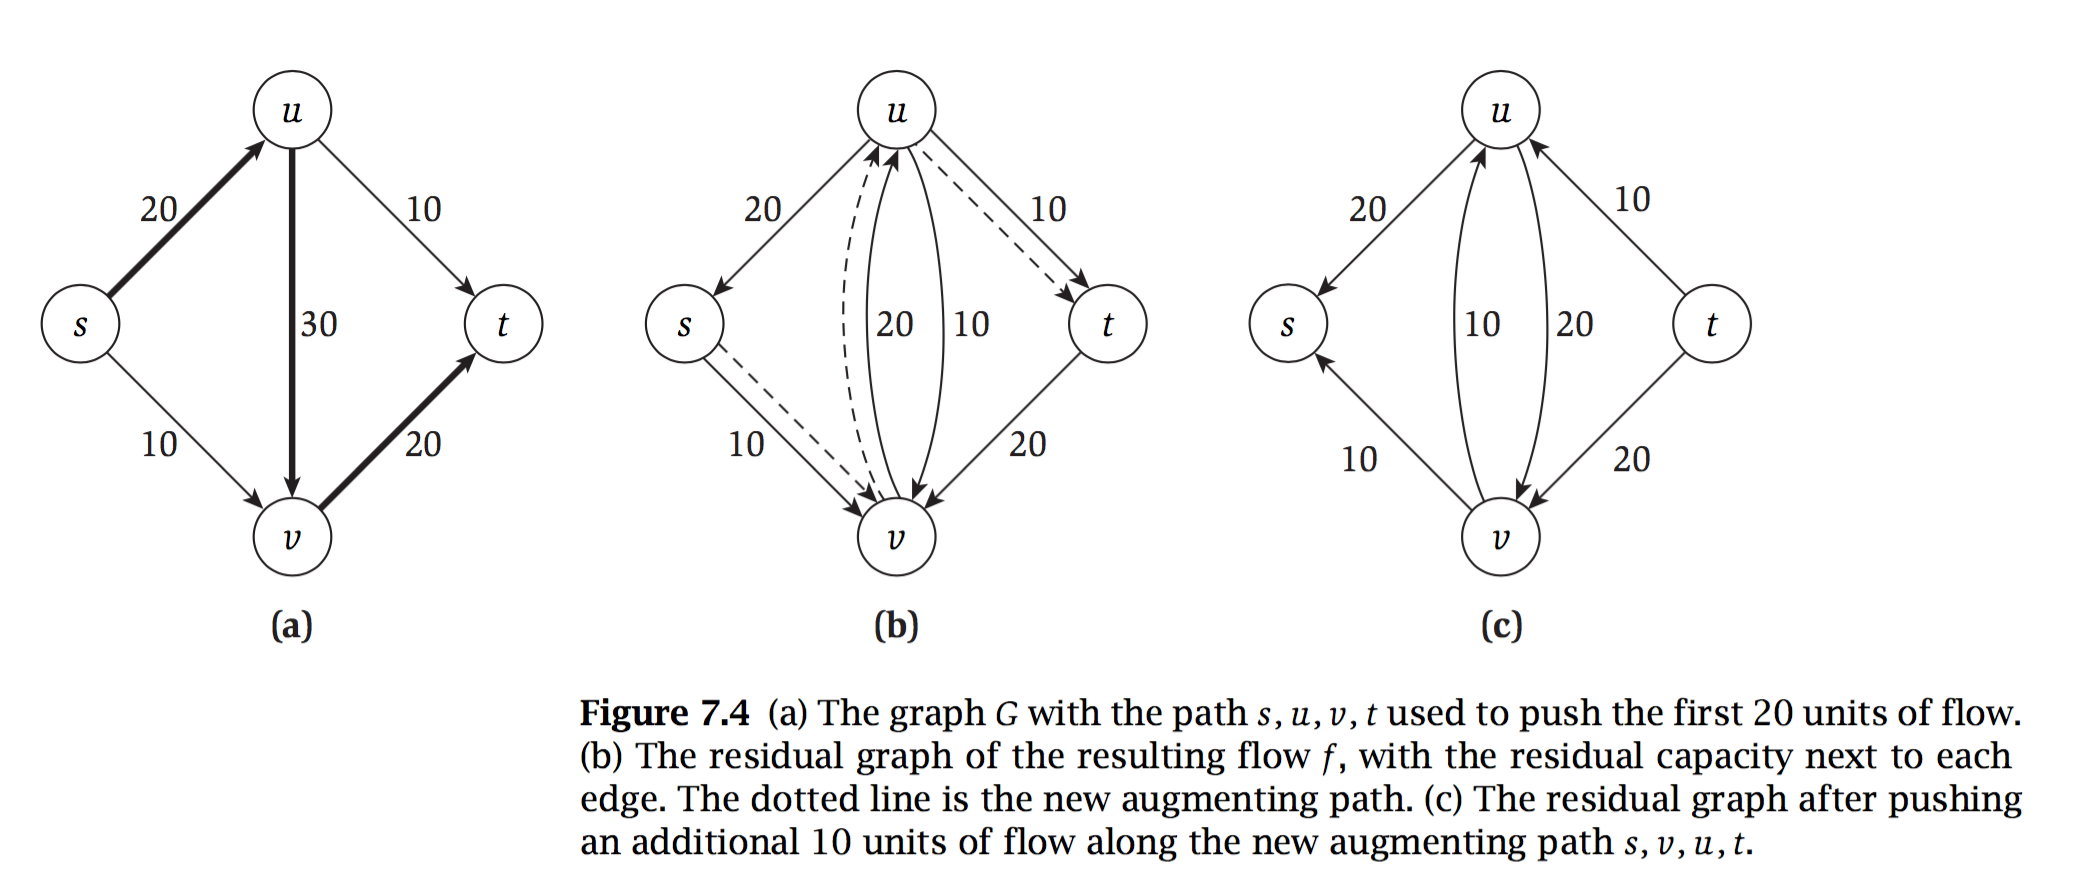
\includegraphics[scale=0.9]{7_4}}
\caption{Flow network and residual graph}
\label{fig:7_4}
\end{figure}
\begin{align*}
&G_R = (V, E')~\text{s.t.}\\
\end{align*}
$G_R$ has the new capacity $C_{GR}$ s.t.
\begin{enumerate}
\item Forward edge: $C_{uv}-f_{uv}$. (leftover)
\item Backward edge:\ $-f_{uv}$. (potential undo amount) 
\end{enumerate}
\subsection{Ford-Fulkserson}
\subsubsection{Algorithm}
\begin{enumerate}
\item Start with $f(e)=0, \forall e \in E$
\item Compute residual graph $G_R$. Strictly $f_{uv}>0$, and forward edge and backward can simultaneously exists. Given a flow $f_{uv} \cdot u \ra v$. 
\begin{itemize}
\item Forward edge capacity: $c_{uv}-f_{uv}$ 
\item Backward edge capacity: $f_{uv}$.
\end{itemize}
\item Find an path $s$-$t$ in $G_R$. 
$$P, \delta(P)=\min_{e\in P} \{C_{G_R}(e)\}$$
strictly, $\delta(R)>0$. 
\item Augment $f$ to get new $f'$, the flow. 
\begin{align}
& f'(uv)= f(uv)+\delta \text{ if $uv\in P$ in a forward edge}\\
& f'(vu)= f(vu)-\delta \text{ if $uv \in P$ in a backward edge} \label{eqn:backward}\\
& f'(uv)=f(uv) \text{ ow}
\end{align}
Notice that in \ref{eqn:backward} is update $vu$, and $uv$ is the backward edge. $f(vu)$ only represents the abs value, not the direction, thus need to $-\delta$. The flow $f(vu)$ and flow $\delta$ are of different directions. 
\item Repeat
\end{enumerate}
\textbf{Proof.} $f'$ is a flow in $G$. The $0\leq f(e)\leq C(e)$. See P343.

\textbf{Proof.} Check conservation condition. 


This algorithm maintains: 
$$
V(f')= V(f)+\delta
$$
Observations:
\begin{enumerate}
\item at $s$, flow $f$ can only hit its out edge - $f^{in}(s)=0$.
\item at $t$, flow $f$ can only hit its in edge - $f^{out}(t)=0$ 
\end{enumerate}
\subsubsection{Termination}
Terminates when \textbf{no residual graph}. The Ford-Fulkerson Algorithm \textbf{terminates}
when the flow $f$ has \textbf{no} $s$-$t$ path in the residual graph $G_R$ (or written
as $G_f$). 


Complexity $O(|E| C_{\text{mincut}})$. 
\subsubsection{Cut}
cut. Let $G_R$ be s.t. $\neg \exists s\sim t$ path. 
\begin{align*}
& A = \{u| s\sim_{G_R} u\} \text{ reachable in graph $G_R$}\\
& B = V/A\\
& \text{cut } (A, B) \sim \text{output}
\end{align*}
, where $V$ is the verticies. 

$(A, B)$ is a cut, iff 
\begin{enumerate}
\item $s\in A, t\in B$. 
\item $A\cap B = \phi$. 
\item $A\cup B = V$
\end{enumerate}
Define $\delta(A,B)=\{uv\in E| u\in A, v\in B\}$. 

Notice: the cut capacity of $cut(A,B)$ is defined as:
$$
cut(A, B) = \sum_{e \text{ out of }A}C(e)
$$

Only consider the edges $A\ra B$, not the edges $A \leftarrow B$. 

\subsubsection{Mincut}
Consider any cut $cut(A,B)$. Cut capacity, natural upper bounds on the values of flows.
\begin{align*}
& Mincut = \min_{cut(A,B)} Cap(A, B)\\
& Maxflow \leq Cap(A, B) \forall A, B \leq Mincut
\end{align*}
To prove $Maxflow = Mincut$. In the residual graph $G_R$:

$$
\max_{flow~f} v(f) = \min_{cut(A, B)} \text{Capacity}(A,B)
$$

\textbf{Proof.} The upper bound of $v(f)$ is mincut. Let $f$ be any flow, $(A,B)$ be any cut. 
\begin{align*}
v(f) &= f^{out}(A)-f^{in}(A) \\
&\leq \sum_{e \text{ out of }A}C(e) - 0\\
&\leq \text{Capacity}(A, B) \\
\end{align*}

This proof does not require any knowledge of Ford-Fulkerson algorithm $\blacksquare$. 

At the time we fail find $s$-$t$ path. The Ford-Fulkerson Algorithm \textbf{terminates} when the flow $f$ has \textbf{no} $s$-$t$ path in the residual graph $G_R$ (or written as $G_f$). 

Consider edge $uv, C(uv)$. See figure \ref{fig:7_5}. 
\begin{align*}
u,v' \in A\\
v,u' \in B \\ 
u \text{ reachable from } s. 
\end{align*}
\begin{figure}[!htp]
\centering
\subfloat{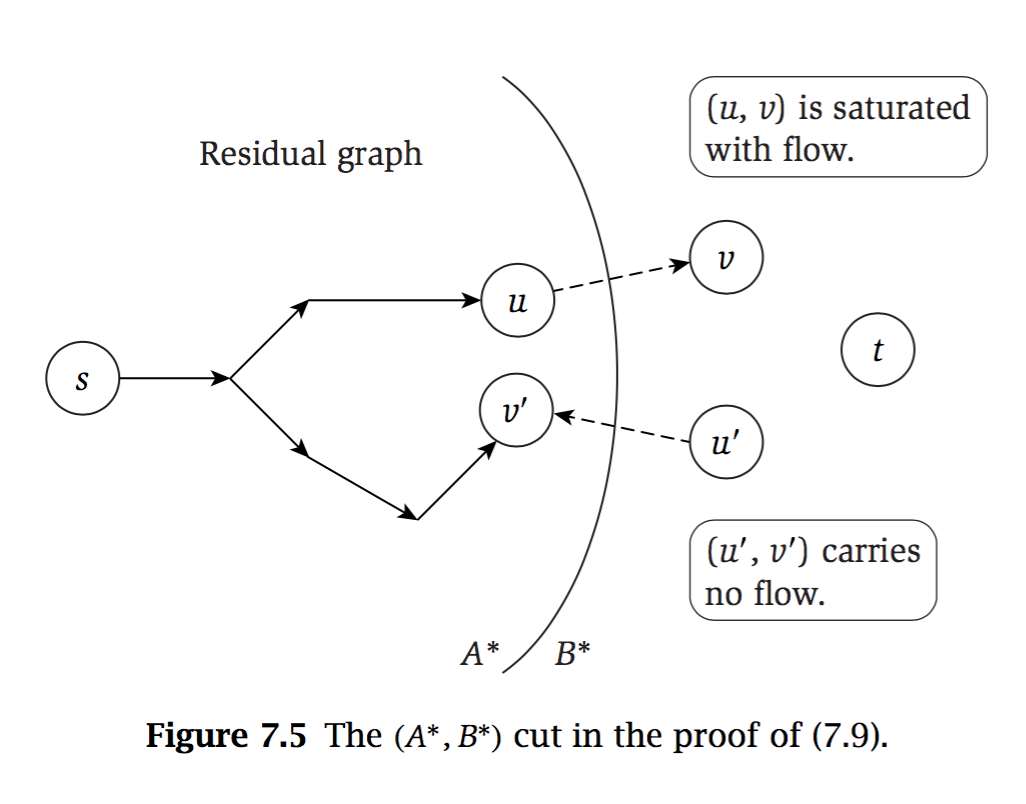
\includegraphics[scale=1.20]{7_5}}
\caption{$Maxflow = Mincut$}
\label{fig:7_5}
\end{figure}

\textbf{Proof}. Prove $f(uv)=C(uv)$. Prove no more positive flow. If there is a $f(uv)< C(uv)$, then there is a \textbf{forward} edge in $G_R$, then $v$ is \textbf{reachable} by $s$; which is contradiction. $\blacksquare$

\textbf{Proof}. Prove $f(u'v')=0$, i.e. proving not flow from $B$ to $A$. (not backward edge in $G_R$). If $(u'v')\neq 0$, it gives rise to \textbf{backward} edge $v'u'$ in $G_R$, then $u'$ is \textbf{reachable} by $s$. Thus contradiction. $\blacksquare$
\subsubsection{Scaling algorithm}
Find the bottleneck of the path, and $\max$ the bottleneck, it can be done by Dijkstra's algorithm. 

Alternatively, increase the performance of FF algorithm. use binary search to boost. 

$\Delta$, the value we want to push on the graph. Let $\Delta=2^t \leq \max C(e)$. Let $\Delta$ be the longest such $\Delta$.
\begin{python}[mathescape]
$f$ = 0
while $\Delta\geq 1$:
  compute $G^\Delta(f)$
  augment $f$ on $G_R$
  update $G_R$
  if not augment:
    $\Delta$/=2
\end{python}
, where $G^\Delta(f)$ filters out that the $e, C(e)\leq \Delta$. 
\subsubsection{Complexity}
$C = \max_{e}C(e)$. The complexity is:
$$
O(|E|(|V|+|E|)\log C) = O(|E|^2 \log C)
$$
, where augment flow, find a path $O(|E|+|V|)$

For every given value $\Delta$, there is at most $O(|E|)$ iterations: 

\begin{align*}
v(f) &= f^{out}(A)-f^{in}(A) \\
&= \sum_{e~out}C(e)-\text{Slack}(e)-f^{in}(A) \\
&\geq \sum_{e~out}C(e)-\sum_{e~out}\Delta-\sum_{e~in}\Delta \\
\\
v(f)+|E|\Delta &\geq \sum_{e~out}C(e) \geq maxflow
\end{align*}

Edmonds-Karp algorithm complexity:
$$
O(|V||E|^2)
$$
\subsection{Applications}
\subsubsection{Maximum Matching - Bipartite Graph}
\begin{figure}[!htp]
\centering
\subfloat{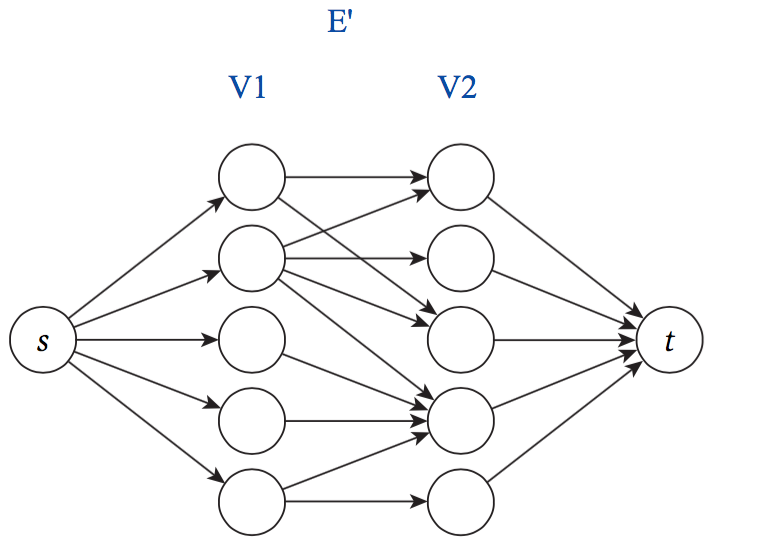
\includegraphics[scale=1.20]{bipart}}
\caption{Bipartite Graph $G$ and $G_\text{Bipart}$}
\label{fig:bipart}
\end{figure}
See figure \ref{fig:bipart}
\begin{align*}
& G_B = (V_1, V_2, E') \\
& G=(V, E) \\
& V= V_1 \cup V_2\cup \{s, t\}\\
& \text{Let } i, j \in V_1 \cup V_2\\
& (i,j)\in E' \leftrightarrow (i, j)\in E\\
& \forall i \in V_1, (s, i) \in E \\
& \forall j \in V_2, (s, j) \in E. 
\end{align*}

Matching. 

\begin{align*}
\forall e \in e, C(e) =1
\end{align*}

\textbf{Proof correspondence}. Let $f$ be any flow of $G$, let $M$ be any matching in $G_B$. Claims:
\begin{enumerate}
\item $\exists$ a matching $M$ s.t. $|M|=v(f)$.

Flow conservation. Select mincut. $\forall v \in V_1\cup V_2$, due to flow conservation, there is only 1 in edge and 1 out edge. $\therefore \forall v_1 \in V_1$ is matched to at most 1 $v_2 \in V_2. $
\item 
\end{enumerate}
\section{Discussion}
\subsection{Job Scheduling}
Do not have node for each time period naively. Use event. 
\subsection{Graph Cohesiveness}
Social network problem. 

\subsection{Matrix Rounding}
\begin{align*}
A_{m\times n} = \begin{bmatrix}
r_{11} & ... & r_{1n} \\
... & &...&\\
r_{m1} & ... & r_{mn}
\end{bmatrix}
\end{align*}
Col sum for $i$-th column: $C_i$; row sum for $i$-th row $R_i$. Overall, the sum of sum are equal: $\sum C_i = \sum R_j$. 

Given $0 \leq r_{ij}\leq 1$. Only the fraction we cares about. 

Think about distribute $\sum R_i$ to the $R_i$ entries, which can only take 0 or 1.

Reduce to max-flow problem. 
\begin{align*}
s \ra \{R_1, ..., R_m\} \ra G \ra \{C_1, ..., C_n\} \ra t
\end{align*}
Can drop the $G$. 
\begin{align*}
s \ra \{R_1, ..., R_m\} \ra \{C_1, ..., C_n\} \ra t
\end{align*}
, vertices with the capacity $R_i, C_j$. 


\textbf{Proof.} Proof correspondence. mat $\Leftrightarrow G$. 

Work from the $V(f)=\sum R_i =\sum C_i$. Each $\{R_1, ..., R_m\}$ and $\{C_1, ..., C_n\}$ are full, and intermediate edges are either 0 or 1. 

\textbf{Proof.} Always $V(f)=\sum R_i$. Find that the \textit{min cut} is the max-flow.
\subsection{Database Projections}
Projection and Permutations.
Columns 1,...,n
\begin{align*}
& S_i \subset \{1,..., n\}\\
& 1 \leq l < k
\end{align*}

Prefix: bag version, order does not matter. e.g.
\begin{align*}
& S_1 = \{3, 5, 1\} \\
& C= \{1, 3,5, 2, 6, 4\}
\end{align*}
One permutation can be used in multiple projections. 

What if two bags, $S_1 \subset S_2$. - 1 permutation.

What if three bags, $S_1 \subset S_2 \subset S_3$. - 1 permutation.

\textbf{Represent the database problem use graph}. Lattice graph: subset relationship of a graph $G$. Boolean lattice.

\begin{align*}
S_1 \ra & S_2 \ra S_5\\
\searrow & S_4 \nearrow
\end{align*}
Partition the graph with minimal number of chain, min cut, the max flow. 
\subsection{Spanning subgraph}
Bipartite \& Undirected
\begin{align*}
s \ra \{L_1, ..., L_m\} \ra G \ra \{R_1, ..., R_n\} \ra t
\end{align*}
For $s \ra L_i$ has as cap $d_{L_i}$. 

Proof necessary condition. 

\section{Project Selection}
\subsection{Construction}
\begin{enumerate}
\item $S$ - set of \textit{project}
\item project $i\in S$, \textit{gain} $P_i$ could be negative 
\item Objective: Select $T\subseteq S$ s.t. $\max \sum_{i\in T} P_i$.
\item Constraint: Directed graph $G=(S, E)$ on projects 
$$
i \ra j
$$
$i$ in selected $\Ra$ $j$ should be selected. Note the graph is directed. Complete $j$ is a necessary condition for starting $i$. 

$T\subseteq S$ in closed, if $i\in T, i\ra j, j \in T$. 
\end{enumerate}
Technique: add $+\infty$ edge weight. 


Consider $\forall i, P_i \geq 0$ and $\forall i, P_i <0$. These special cases are shown below:

\begin{figure}[!htp]
\centering
\subfloat{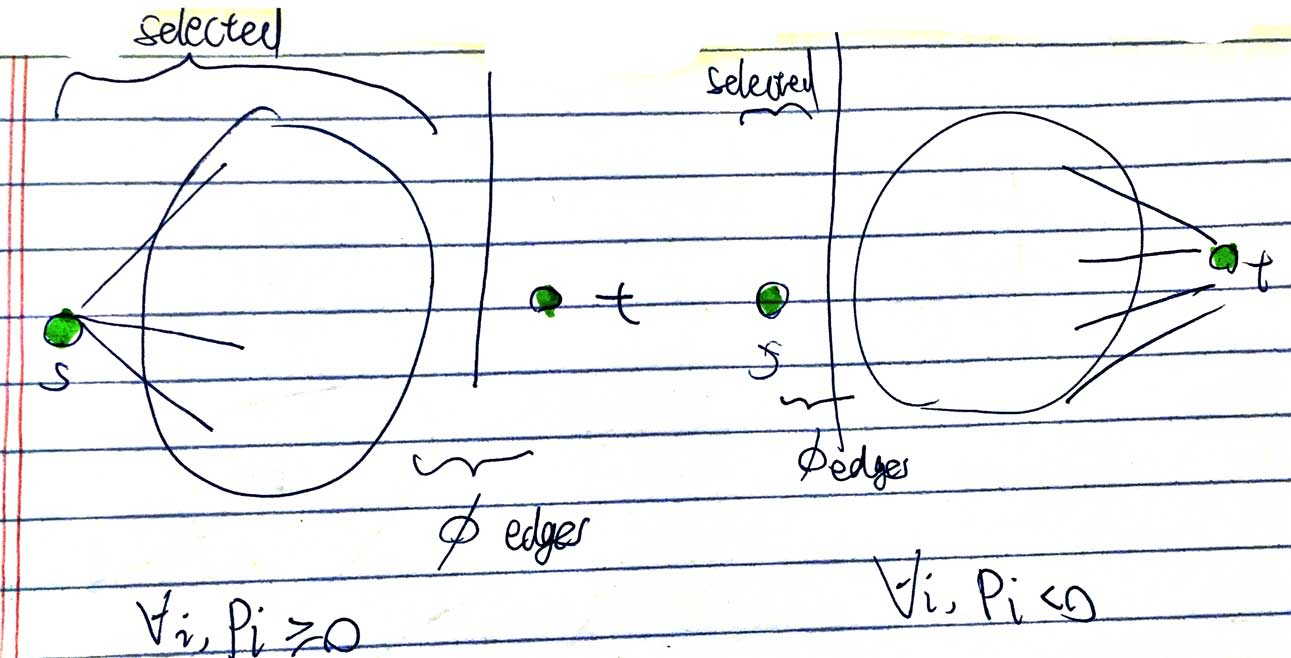
\includegraphics[scale=1.10]{scheduleprojectSpecial}}
\caption{Degenerated cases}
\label{fig:scheduleprojectSpecial}
\end{figure} 

\subsection{Proof}

$+\infty$ capacity, then cannot be mincut, since $\exists$ cut with finite value.

In general case. 

\begin{figure}[!htp]
\centering
\subfloat{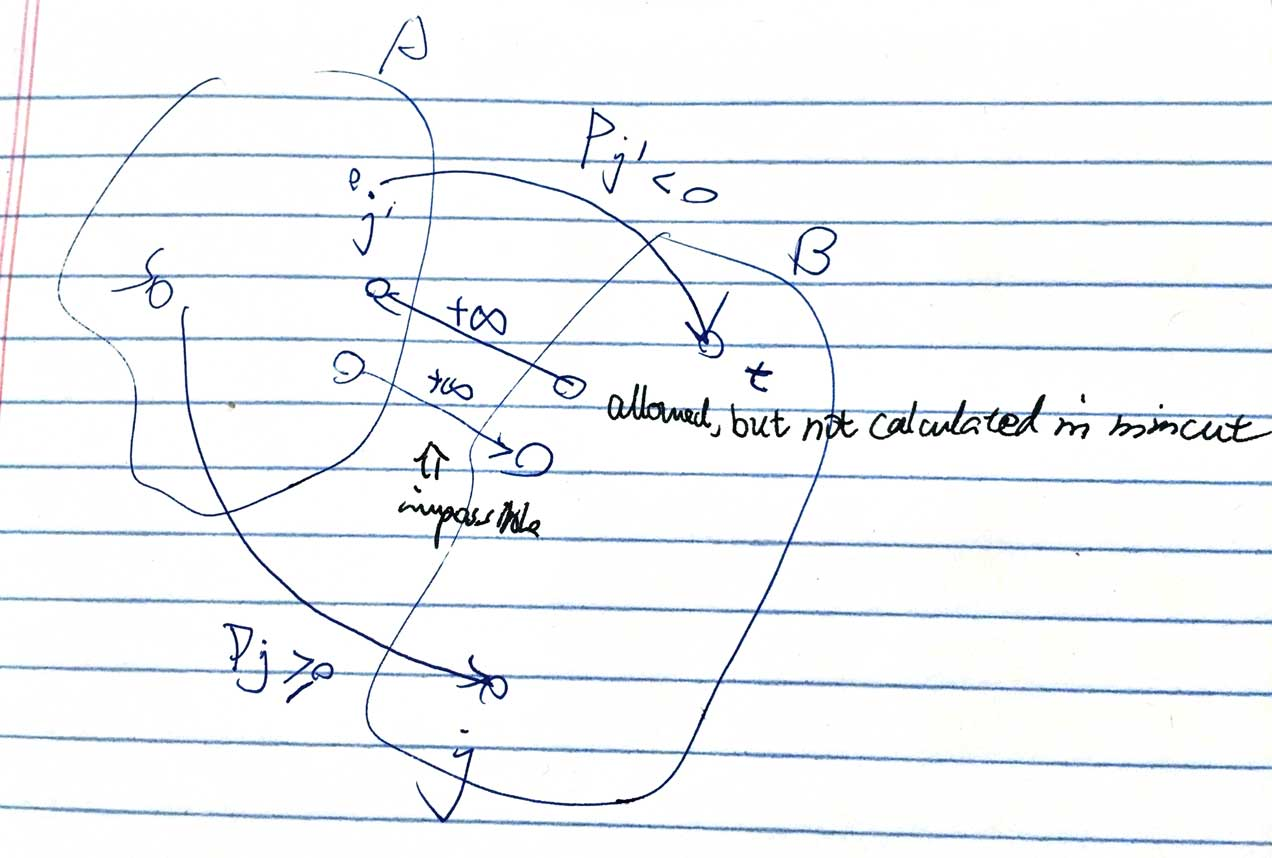
\includegraphics[scale=1.20]{scheduleproject}}
\caption{Schedule Project}
\label{fig:scheduleproject}
\end{figure}

$Cap(A, B)=\sum_{e~out~A} = \sum_{j \notin A, P_j\geq 0}P_j+\sum_{j \in A, P_j<0}-P_j$. If $j \notin A, j$ is connected to $s$. If $j \in A, j$ is connected to $t$. 

$T=A/\{s\}$.

\begin{align*}
Cap(A, B)&=\sum_{j\notin T, P_j\geq 0}P_k+\sum_{j\in T, P_j <0}(-P_j) \\
&= (\sum_{P_j\geq 0}P_j-\sum_{j \in T, P_j\geq 0}P_j)+\sum_{j\in T, P_j <0}-P_j.\\
&=  \sum_{P_j\geq 0}P_j - Profit(T)
\end{align*}

, where $\sum_{P_j\geq 0}P_j$ is a constant.

Therefore, max the profit T $\equiv$ min the cut of #Cap(A, B). The correspondence is proved. 


\section{Baseball Elimination}
\begin{enumerate}
\item $S$ - collection of teams 
\item $x\in S, w_x$ number of of wins
\item $x, y \in S, g_{x, y}$  \# of games to be played (more games to play)
\item For a given, $z\in S$ specific team, $m$ \# of possible wins. $m \leq w_z+\sum_{x\in S} g_{z,x}$
\end{enumerate}

Describe the \textbf{middle} of seasons. undirected graph

Team and $w_j$ - NY: 92, BLT: 91, TNT: 91, BOS: 90.

$$x -\ _{g_{x, y}} - y$$


Under this notation, we have developed a very rudimentary graph: 
\begin{figure}[!htp]
\centering
\subfloat{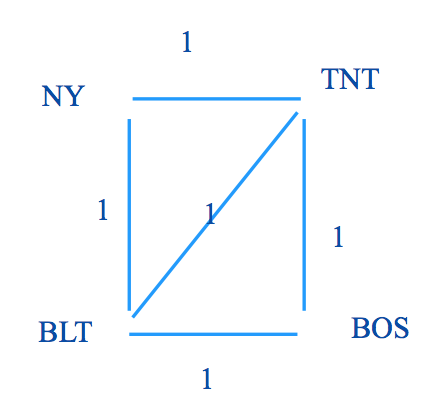
\includegraphics[scale=1.20]{baseball0}}
\caption{Graph with edge of $g_{x,y}$}
\label{fig:baseball0}
\end{figure}
\subsection{Construction}
From the $z$'s perspective. 

$s$ sends $g_{x,y}$, on pair $(x,y)$, then split the wins, then $t$ constrains number of wins. 

\begin{figure}[!htp]
\centering
\subfloat{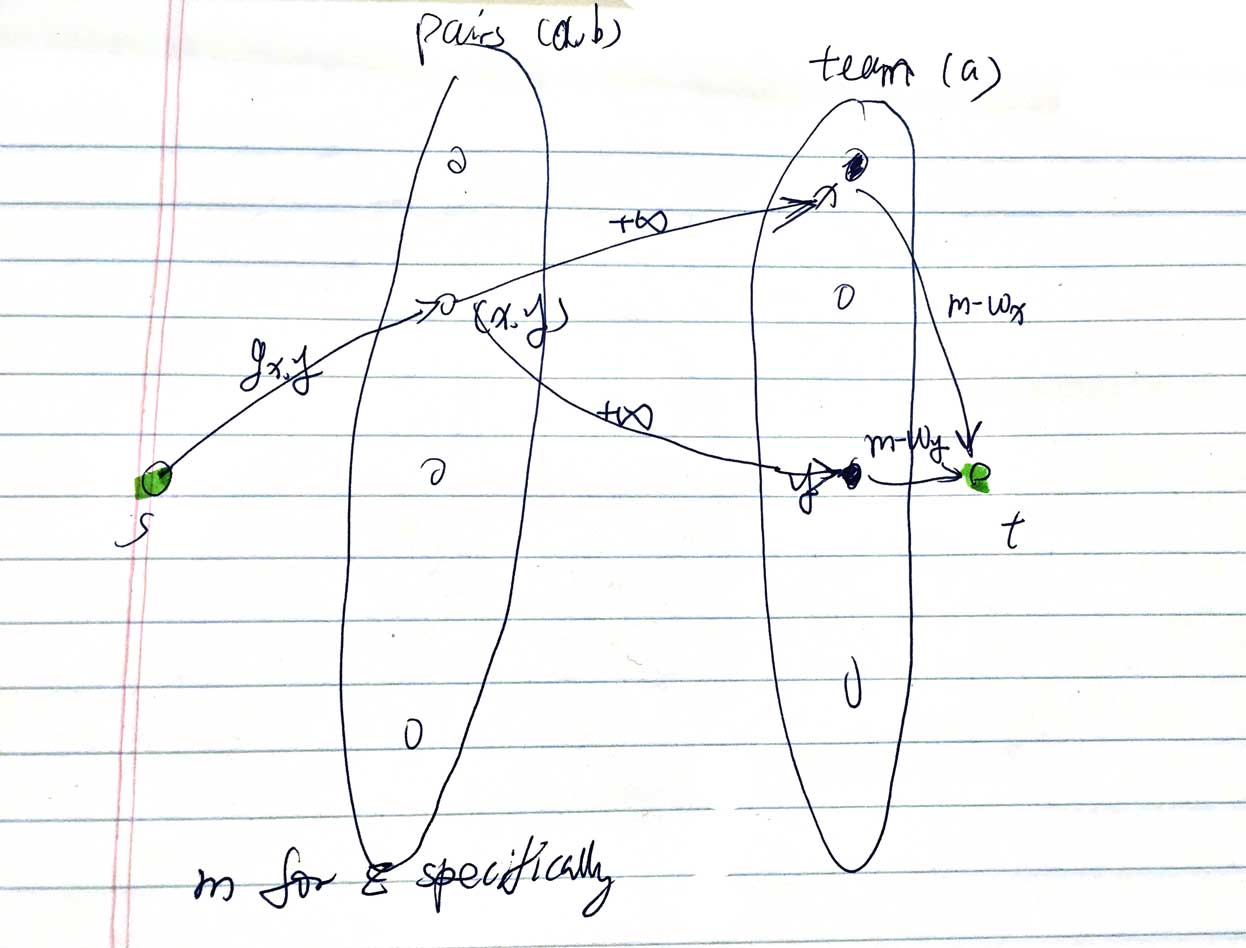
\includegraphics[scale=1.0]{baseball01}}
\caption{Network construction}
\label{fig:baseball01}
\end{figure}

\subsection{Proof}
\begin{figure}[!htp]
\centering
\subfloat{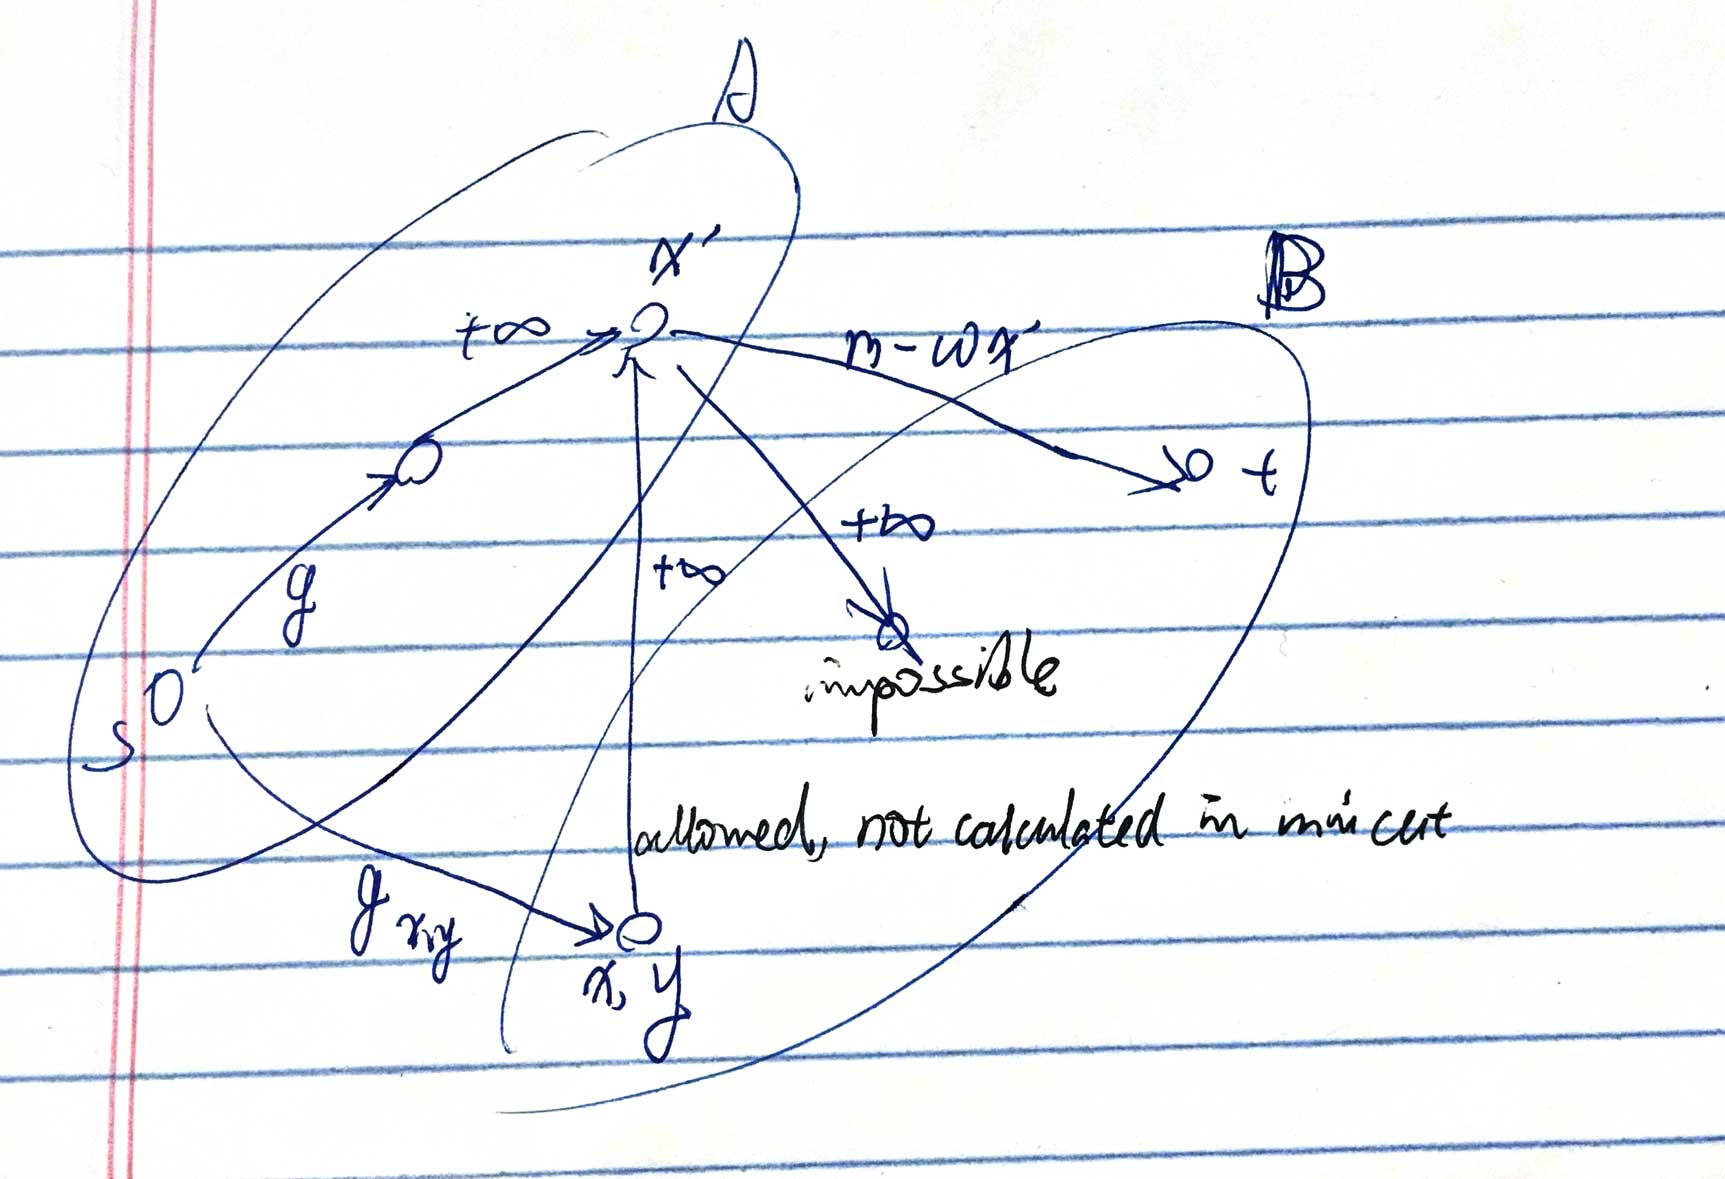
\includegraphics[scale=.90]{baseball}}
\caption{Baseball Elimination}
\label{fig:baseball}
\end{figure}
Let $g^*=\sum_{(x,y)} g_{x, y}$. $maxflow = g^*$? If $\neq$, $z$ cannot win $m$. 

Let $(A, B)$ be a cut.
\begin{align*}
Cap(A, B) &= \sum_{(x,y)\notin A} g_{x,y}+\sum_{x\in T} m-w_x\\
&= \sum_{(x,y)}g_{x, y}-\sum_{(x, y)\in A} g_{x, y}+\sum_{x\in T}m-w_x\\
&= g^*-\sum_{(x, y)\in A} g_{x, y}+m|T|\sum_{x\in T}-w_x
\end{align*}
, where $T=$ teams $\in A$.

If $maxflow <g^*$, $m=(\sum_{x\in T} w_x+\sum_{(x,y)\in A} g_{x,y})/|T|$. i.e. the average win played among teams except $z$ themselves. 

\textbf{Proof.} $(x,y)\in A$, then $x, y\in T$. If $x \notin T$, then $x \in B$, then $\exists e$ that connects $(x,y)\in A$ and $x\in B$, thus mincut $+\infty$, which contradicts the fact that the mincut is finite $\blacksquare$. 

\textbf{Eliminate $z$}. 
\begin{itemize}
\item $z$ can finish with at most $m$ wins.
\item $\exists T\subseteq S$ so that
$$
\sum_{x\in T} w_x + \sum_{x, y \in T} g_{x, y} > m|T|
$$
The average \#wins in $T$ is larger than $m$. $\therefore \exists t \in T$, a team ends with strictly more than $m$ wins. $\therefore z$  can be eliminated.
\end{itemize}

\subsection{Social cohesiveness}
This problem is similar to problem of baseball elimination. 

Application, community detection in FB\ social network graph.

\subsection{Spanning Subtree}
$G=(V_1, V_2, E)$. Bipartie. Subgraph, $G'=(V_1, V_2, E')$, where $E'\subseteq E$.

Degree $deg(v)=|\{uv|u\in V_1\cup V_2\}|$. 

Property of the degree $\sum_v deg(v)=2|E|$

\subsection{Database projection}
Cover the graph with the minimum number of chains. After you select a vertex on the chain, the vertex can only be selected \textbf{once}. $\forall v\in V, f^{out}(v)=f^{in}(v)=1$, 
\end{document}
